\documentclass[12pt]{article}

\usepackage[danish]{babel}
\usepackage{latexsym, amsfonts, amssymb, amsthm, amsmath}
\usepackage{siunitx}
\usepackage{graphicx, pgfplots}
\usepackage{sagetex}

%loaded last
\usepackage[hidelinks]{hyperref}

\sisetup{exponent-product = \cdot,
  output-decimal-marker = {,}}

%Giles Castelles incfig
\usepackage{import}
\usepackage{xifthen}
\usepackage{pdfpages}
\usepackage{transparent}

\newcommand{\incfig}[2][1]{%
  \def\svgwidth{#1\columnwidth}
  \import{../figures/}{#2.pdf_tex}
}

\setlength{\parindent}{0in}
\setlength{\oddsidemargin}{0in}
\setlength{\textwidth}{6.5in}
\setlength{\textheight}{8.8in}
\setlength{\topmargin}{0in}
\setlength{\headheight}{18pt}

\pgfplotsset{compat=newest}

\pgfplotsset{every axis/.append style={
  axis x line=middle,    % put the x axis in the middle
  axis y line=middle,    % put the y axis in the middle
  axis line style={<->,color=black}, % arrows on the axis
}}

\title{Opgaver til forelæsning 16}
\author{Noah Rahbek Bigum Hansen}
\date{26. Oktober 2024}

\begin{document}

\maketitle

\section*{Opg. 10.45}
\textbf{The Spinning Figure Skater}. The outstretched hands and arms of a figure skater preparing for a spin can be considered a slender rod pivoting about an axis through its center. When the skater’s hands and arms are brought in and wrapped around his body to execute the spin, the hands and arms can be considered a thin-walled, hollow cylinder. His hands and arms have a combined mass of \qty{8,0}{kg}, When outstretched, they span \qty{1,8}{m}; when wrapped,m they form a cylinder of radius \qty{25}{cm}. The moment of inertia about the rotation axis of the remainder of his body is constant and equal to \qty{0,40}{kg\cdot m^2}. If his original angular speed is \qty{0,40}{rev/s} , what is his final angular speed?
\bigbreak
Først findes inertimomentet af skøjteløberens arme idet disse antages at kunne modeleres som en solid stand med jævnfordelt masse. Altså har vi at
\[
I_{a_0} = \frac{1}{12}ML^2 = \frac{1}{12}\cdot \qty{8,0}{kg} \cdot \left( \qty{1,8}{m}  \right)^2 = \qty{2,16}{kg\cdot m^2} 
.\]
Altså bliver det samlede inertimoment med udstrukne arme
\[
I_0 = I_{a_0} + I = \qty{2,16}{kg\cdot m^2} + \qty{0,40}{kg\cdot m^2} = \qty{2,56}{kg\cdot m^2} 
.\]
Idet skøjteløberen trækker armene til sig falder inertimomentet af armene til
\[
I_{a_1} = MR^2 = \qty{8,0}{kg} \cdot \left( \qty{25}{cm}  \right)^2 = \qty{0,5}{kg\cdot m^2} 
.\]
Altså er det samlede inertimoment med armene ind til kroppen
\[
I_1 = I_{a_1} + I = \qty{0,9}{kg\cdot m^2} 
.\]
Idet vi fra formlen for impulsmoment har at $I \sim \omega^{-1}$ må det gælde at
\[
\frac{I_0}{I_1} = \frac{\omega_1}{\omega_0} \implies \omega_1 = \frac{\omega_0 \cdot I_0}{I_1} = \frac{\qty{0,40}{\frac{rev}{s}} \cdot \qty{2,56}{kg\cdot m^2} }{\qty{0,9}{kg\cdot m^2} } = \qty{1,14}{\frac{rev}{s}} 
.\]




\section*{Opg. 10.49}
A small \qty{10,0}{g} bug stands at one end of a thin uniform bar that is initially at rest on a smooth horizontal table. The other end of the bar pivots about a nail driven into the table and can rotate freely, without friction. The bar has mass \qty{50,0}{g} and is \qty{100}{cm} in length. The bug jumps off in the horizontal direction, perpendicular to the bar, with a speed of \qty{20,0}{cm/s} relative to the table. 

\subsection*{(a)}
What is the angular speed of the bar just after the frisky insect leaps?
\bigbreak
Baren modelleres som en tynd pind med omdrejningsakse om den ene af dens ender. Altså har denne et inertimoment på
\[
I = \frac{1}{3}ML^2 = \frac{1}{3}\cdot \qty{50,0}{g} \cdot (\qty{100}{cm})^2 = \qty{0,0167}{kg.m^2} 
.\]
Impulsmoment, $L$, er en konserveret størrelse og da der er stilstand inden insekten hopper må det altid gælde at $L=0$. Derfor må det gælde at
\[
  L_1 + L_2 = 0    
,\]
hvor $L_1$ er insektens impulsmoment og $L_2$ er stangens ditto. Disse er givet ved hhv.
\begin{align*}
  L_1 &= m\cdot v\cdot l = \qty{10,0}{g} \cdot \qty{20,0}{\frac{cm}{s}} \cdot \qty{100}{cm} = \qty{2e-3}{m^2.kg.s^{-1}}   \\
  L_2 &= I\omega \implies \omega = \frac{L_2}{I}\\
\end{align*}
Altså får vi at
\[
  \omega = \frac{- \qty{2e-3}{kg.m^2.s^{-1}}}{\qty{0,0167}{kg.m^2}} = \qty{-0,120}{s^{-1}} 
.\]


\subsection*{(b)}
What is the total kinetic energy of the system just after the bug leaps?
\bigbreak
Den kinetiske energi omfatter både translatorisk og rotationel energi. Altså er den samlede kinetiske energi summen af insektets translatoriske energi (denne har en rotationel energi på 0) og stangens rotationelle energi (denne har en translatorisk energi på 0). Altså får vi at
\begin{align*}
  k_1 &= \frac{1}{2}m\cdot v^2 + \frac{1}{2}I\omega^2 \\
  &= \frac{1}{2}\left( \qty{10,0}{g} \cdot \left( \qty{20,0}{cm.s^{-1}}\right)^2 + \qty{0,0167}{kg.m^2}\cdot \left( \qty{-0,120}{s^{-1} }  \right)^2   \right) = \qty{3,2e-4}{J}  
\end{align*}


\subsection*{(c)}
Where does this energy come from?
\bigbreak
Denne energi kommer fra insektens muskler i benene som den brugte til at hoppe med.

\section*{Opg. 10.51}
You live on a planet far from ours. Based on extensive communication with a physicist on earth, you have determined that all laws of physics on your planet are the same as ours and you have adopted the same units of seconds and meters as on earth. But you suspect that the value of $g$, the acceleration of an object in free fall near the surface of your planet, is different from what it is on earth. To test this, you take a solid uniform cylinder and let it roll down an incline. The vertical height $h$ of the top of the incline above the lower end of the incline can be varied. You measure the speed $v_{cm}$ of the center of mass of the cylinder when it reaches the bottom for various values of $h$. You plot $v_{cm}^2$ (in $\unit{\frac{m^2}{s^2}}$) versus $h$ (in $\unit{m}$) and find that your data lie close to a straight line with a slope of $\qty{6,42}{\frac{m}{s^2}}$. What is the value of $g$ on your planet?
\bigbreak
Fra konservation af energi har vi at
\begin{align*}
  k_1 + U_1 &= k_2 + U_2 \\
  Mgh  + 0 &= \frac{1}{2}m\cdot v_{cm}^2 \frac{1}{2}\cdot I\cdot \omega^2 + 0 \\
  &= \frac{1}{2}M\cdot v_{cm}^2 + \frac{1}{2}\cdot \frac{1}{2}MR^2\left( \frac{v_{cm}}{R}  \right)^2    \\
  &= \frac{1}{2}M\cdot v_{cm}^2 + \frac{1}{4}M\cdot v_{cm}^2  \\
  &= \frac{3}{4}M\cdot v_{cm}^2 \\
  g &= \frac{3}{4} \frac{v_{cm}^2}{h} = \frac{3}{4}\cdot \qty{6,42}{m.s^{-2}} = \qty{4,82}{m.s^{-2}}
\end{align*}


\section*{Opg. 10.73}
\begin{figure} [ht]
  \centering
  \caption{}
  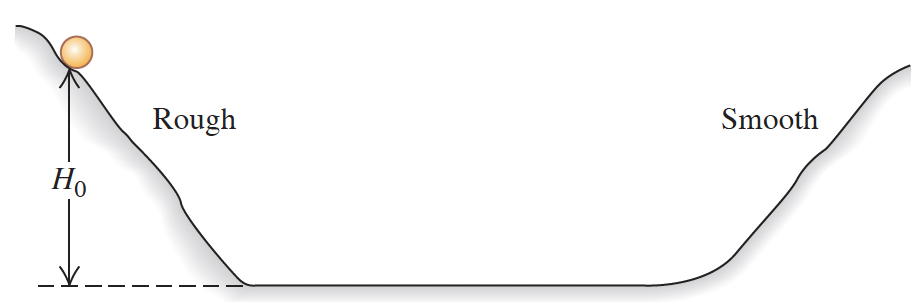
\includegraphics[width=0.5\linewidth]{../figures/P10_73.png}
  \label{fig:P10_73}
\end{figure}

A basketball (which can be closely modeled as a hollow spherical shell) rolls down a mountainside into a valley and then up the opposite side, starting from rest at a height $H_0$ above the bottom. In \textbf{\autoref{fig:P10_73}}, the rough part of the terrain prevents slipping while the smooth part has no friction. Neglect rolling friction and assume the system’s total mechanical energy is conserved.

\subsection*{(a)}
How high, in terms of $H_0$, will the ball go up the other side?
\bigbreak
Energikonservation siger at
\begin{align*}
  k_{0} + U_{0} &= k_{1} + U_{1} \\
  0 + MgH_0 &= \frac{1}{2}M\cdot v^2 + \frac{1}{2}I\omega^2 + 0 \\
  MgH_0 &= \frac{1}{2}M\cdot v^2 + \frac{1}{2}\cdot \frac{2}{3}MR^2 \left( \frac{v}{R}  \right)^2 \\
  gH_0 &= \frac{1}{2}v^2 + \frac{1}{3}v^2 = \frac{5}{6}v^2\\
  v^2 &= \frac{6}{5}gH_0 
\end{align*}
Nu har vi et udtryk for hastigheden af basketbolden når den når ned i bunden af dalen. Energikonservation foreskriver at alt dette omdannes til potentiel energi igen på vej op ad den anden side idet der ikke er nogen friktion. Altså får vi at
\begin{align*}
  U_{2} &= k_{1} \\
  Mgh &= \frac{1}{2}M\cdot \frac{6}{5}gH_0 \\
  h &= \frac{3}{5}H_0
\end{align*}



\subsection*{(b)}
Why doesn’t the ball return to height $H_0$? Has it lost any of its original potential energy?
\bigbreak
Bolden returnerer ikke til sin oprindelige højde, da den stadig har rotationel energi når den når sin maksimale højde på den glatte side. Denne rotationelle energi kan ikke omdannes til potentiel energi, da der ikke er nogen friktion.

\end{document}
